%% using aastex version 6.2
\documentclass[RNAAS]{aastex62}

%% The default is a single spaced, 10 point font, single spaced article.
%% There are 5 other style options available via an optional argument. They
%% can be envoked like this:
%%
%% \documentclass[argument]{aastex62}
%% 
%% where the layout options are:
%%
%%  twocolumn   : two text columns, 10 point font, single spaced article.
%%                This is the most compact and represent the final published
%%                derived PDF copy of the accepted manuscript from the publisher
%%  manuscript  : one text column, 12 point font, double spaced article.
%%  preprint    : one text column, 12 point font, single spaced article.  
%%  preprint2   : two text columns, 12 point font, single spaced article.
%%  modern      : a stylish, single text column, 12 point font, article with
%% 		  wider left and right margins. This uses the Daniel
%% 		  Foreman-Mackey and David Hogg design.
%%  RNAAS       : Preferred style for Research Notes which are by design 
%%                lacking an abstract and brief. DO NOT use \begin{abstract}
%%                and \end{abstract} with this style.
%%
%% Note that you can submit to the AAS Journals in any of these 6 styles.
%%
%% There are other optional arguments one can envoke to allow other stylistic
%% actions. The available options are:
%%
%%  astrosymb    : Loads Astrosymb font and define \astrocommands. 
%%  tighten      : Makes baselineskip slightly smaller, only works with 
%%                 the twocolumn substyle.
%%  times        : uses times font instead of the default
%%  linenumbers  : turn on lineno package.
%%  trackchanges : required to see the revision mark up and print its output
%%  longauthor   : Do not use the more compressed footnote style (default) for 
%%                 the author/collaboration/affiliations. Instead print all
%%                 affiliation information after each name. Creates a much
%%                 long author list but may be desirable for short author papers
%%
%% these can be used in any combination, e.g.
%%
%% \documentclass[twocolumn,linenumbers,trackchanges]{aastex62}
%%
%% AASTeX v6.* now includes \hyperref support. While we have built in specific
%% defaults into the classfile you can manually override them with the
%% \hypersetup command. For example,
%%
%%\hypersetup{linkcolor=red,citecolor=green,filecolor=cyan,urlcolor=magenta}
%%
%% will change the color of the internal links to red, the links to the
%% bibliography to green, the file links to cyan, and the external links to
%% magenta. Additional information on \hyperref options can be found here:
%% https://www.tug.org/applications/hyperref/manual.html#x1-40003
%%
%% If you want to create your own macros, you can do so
%% using \newcommand. Your macros should appear before
%% the \begin{document} command.
%%
\newcommand{\vdag}{(v)^\dagger}
\newcommand\aastex{AAS\TeX}
\newcommand\latex{La\TeX}

\received{\today}
\revised{\today}
\accepted{\today}
\submitjournal{RNAAS}

\shorttitle{B1937+21 Giant Pulse}
\shortauthors{Foster and Karastergiou}

\begin{document}

\title{A Giant Pulse detected from B1937+21 during LOFAR-UK Observations}

\correspondingauthor{Griffin Foster}
\email{griffin.foster@physics.ox.ac.uk}

\author[0000-0002-7559-4291]{Griffin Foster}
\affil{University of Oxford, Sub-Department of Astrophysics \\
Denys Wilkinson Building, Keble Road \\
Oxford, OX1 3RH, United Kingdom}

\author{Aris Karastergiou}
\affil{University of Oxford, Sub-Department of Astrophysics \\
Denys Wilkinson Building, Keble Road \\
Oxford, OX1 3RH, United Kingdom}
\affil{Physics Department, University of the Western Cape\\
Cape Town 7535, South Africa}
\affil{Department of Physics and Electronics, Rhodes University\\
PO Box 94, Grahamstown 6140, South Africa}

\keywords{pulsars: individual B1937+21, scattering, radio continuum: general}

\section{}

% * cordes frbs from pulsars

A Giant Pulse (GP) from B1937+21 \citep{1982Natur.300..615B} was detected during
observations with the LOFAR-UK station using the ARTEMIS
\citep{2015MNRAS.452.1254K} pulse detection back-end at 2016-06-20 01:46:32.457
UTC. The detection occurred using the high-band array (HBA) centred at 145~MHz
with a bandwidth of $5.85$~MHz.

After initial detection the dynamic spectrum was incoherently de-dispersed with
a Dispersion Measure (DM) of $71.0237$~pc~cm$^{-3}$.  The time series of the
pulse is shown in Figure \ref{fig:pulse}.  B1937+21 has a period of $1.56$~ms
and a pulse width of $38.2~\mu$s.  The data is time smoothed using a boxcar
function to a resolution of $2.6$~ms. We assume the measured profile is from a
single GP that is scattered over multiple pulse periods.

%The system equivalent flux density (SEFD) of an international station HBA is
%measured to be approximately 1900~Jy over the observed region of the band
%\footnote{https://www.astron.nl/radio-observatory/astronomers/lofar-imaging-capabilities-sensitivity/sensitivity-lofar-array/sensiti}.
%Using the radiometer equation results in a system noise of approximately 14~Jy
%at a time resolution of $2.6$~ms and bandwidth $5.8$~MHz. The scattered pulse has
%a measured peak flux of approximately 131~Jy.
The sensitivity of an international station HBA beam used during ARTEMIS
observations was measured to be $\sigma_s = 27$~Jy for a $5.85$~MHz band at
145~MHz at a resolution of $327.68 \mu$s \citep{2015MNRAS.452.1254K}.
Integrating the time resolution by a factor of 8 to $2.6$~ms results in a
station sensitivity of $\sigma_s = 9$~Jy. The scattered pulse has a measured
peak flux density $S_{\textrm{peak,scattered}} = 80 \pm 9$~Jy.

An isotropic scattering model \citep{2017MNRAS.470.2659G} was fit to the pulse
resulting in a fit scattering time scale $\tau_{\textrm{iso}}$ of $3.2 \pm
0.3$~ms consistent with the expected scattering using the NE2001
\citep{2002astro.ph..7156C} model of $3.27$~ms. The fit for the pulse before
scattering has a peak flux density $S_{\textrm{peak,iso}} =167 \pm 21$~Jy and is
unresolved in width as expected.

% aslxlap07:~/local/data/LOFAR/B1937+21/B1937+21.ipynb
\begin{figure}
	\centering
    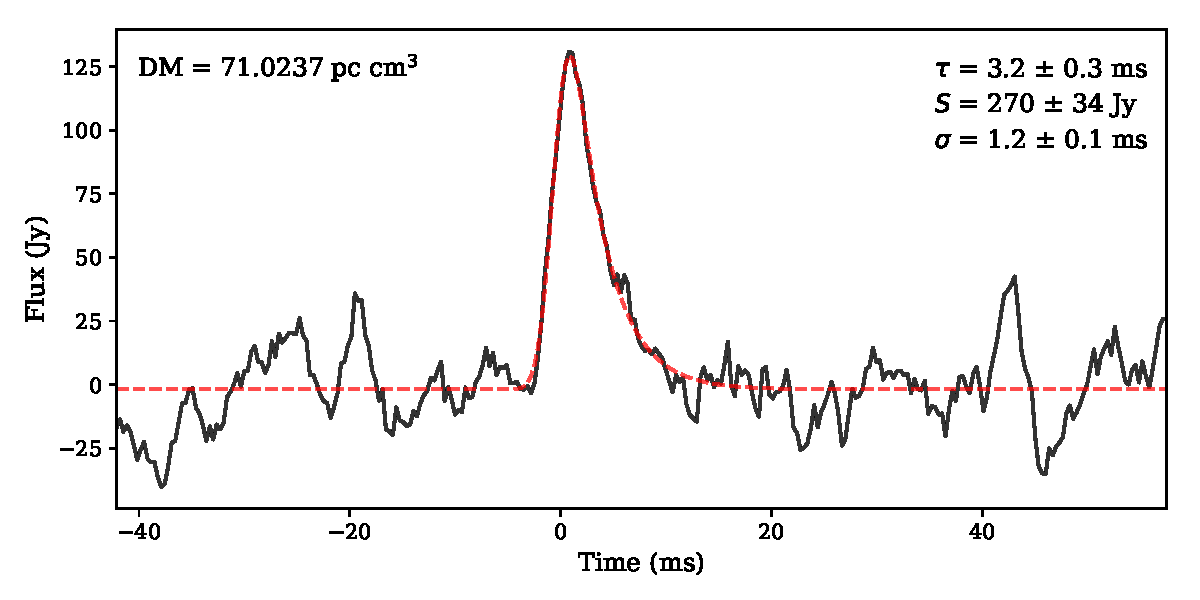
\includegraphics[width=0.75\linewidth]{figures/B1937+21_pulse.pdf}
    \caption{Time series of a giant pulse from B1937+21 (black solid), the data
    has been de-dispersed by the catalogue DM and smoothed with a boxcar filter
    to a time resolution of $2.6$~ms. An isotropic scattering model has been fit
    to the pulse (red dashed). The best fit model parameters are presented in
    the upper right corner.
    }
    \label{fig:pulse}
\end{figure}

\cite{2016A&A...585A.128K} reported detection of B1937+21 at frequencies below
200~MHz but reported no GP detections. The mean flux density was measured to be
$S_{\textrm{mean}} = 370$~mJy over the HBA band. The flux density of the GP
reported here is approximately 200 times brighter than the mean flux density.

\cite{2002AstL...28...21K} reported the detection of four GP's at 112~MHz
ranging from $8.5 - 10$~Jy in peak flux density. The peak flux density of the
pulse reported here exceeds these flux densities by approximately an order of
magnitude. But, as these detections occurred at lower frequencies the pulses
were more scattered.  The intrinsic peak flux density can be computed using
$S_{\textrm{peak,intrinsic}} = S_{\textrm{peak,iso}} \frac{W50_{GP}}{\Delta t}$.
Where $\Delta t=2.6$~ms is time series resolution as the pulse is unresolved and
$W50_{GP} = 10~\mu$s is the measured GP pulse width from higher frequency
observations \citep{2000ApJ...535..365K}. Using this equation, the intrinsic
peak flux density of the detected pulse is approximately 44000~Jy.

This is the only pulse detected from B1937+21 over the extent of the ARTEMIS
observing program. A total of 3000~hours of observing has been performed, during
a 24-hour period B1937+21 transits a beam for approximately 12 minutes,
resulting in a total of approximately 1 day of observing time on B1937+21. We
set an upper limit on the GP event rate from pulses with a minimum peak flux
density of 80~Jy $(S_{\textrm{peak}} \geq 80~\textrm{Jy})$ to one per day at
these frequencies, or once every 55 million pulse periods.

The dynamic spectrum data and analysis notebook is available on
github\footnote{https://github.com/griffinfoster/B1937-21-GP-Note}.

\bibliographystyle{aasjournal}
\bibliography{refs}

\end{document}
